\documentclass[a4paper,10pt,twocolumn]{article}
\usepackage[T1]{fontenc}
\usepackage[utf8]{inputenc}
\usepackage[italian]{babel}
\usepackage[top=3cm, bottom=3cm, left=2.5cm, right=2.5cm]{geometry}
\usepackage{graphicx}
\graphicspath{ ./images/} 
\usepackage{subfig}
\usepackage{dblfloatfix}


\begin{document}

\title{SIR Simulation}
\author{Lorenzo Manini \and Nicolò Montalti}
\date{A.A. 2019/2020}

\maketitle

\section{Descrizione del progetto}
\section{Compilazione ed esecuzione}

%ambiente per codice
\begin{verbatim}
    cmake ..
    make
\end{verbatim}

\section{Risultati}
L'applicazione restituisce due tipi di output grafici. In una finestra vengono mostrate le persone, schematizzante come cerchi colorati, che si muovono in uno spazio quadrato. Lo stato delle persone è rappresentato con colori diversi: verde per i sani, rosso per gli infettivi, arancione per le persone in incubazione, bianco per quelle in quarantena e blu per i recuperati. Un'immagine d'esempio è mostrata in fig. \ref{fig:display}.

\begin{figure}
    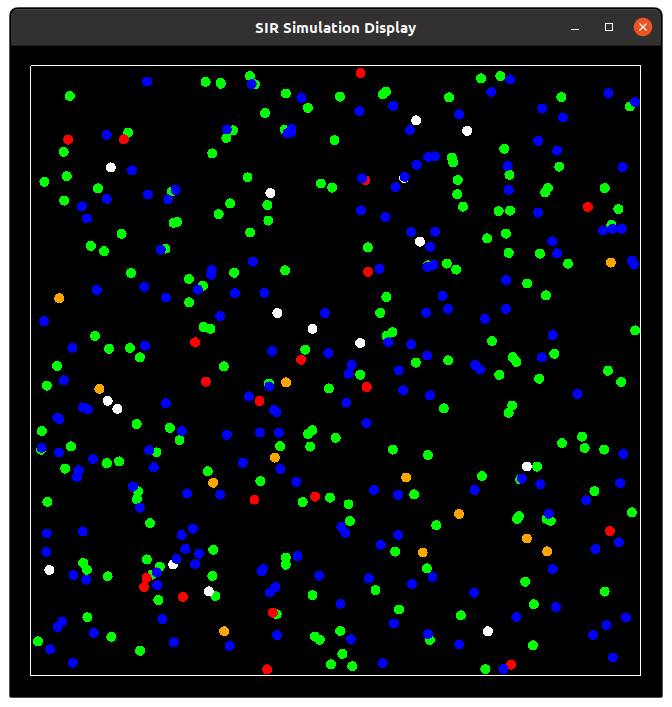
\includegraphics[width=\linewidth]{images/display.png}
    \caption{Finestra grafica ottenuta dalla classe Display. Il verde corrisponde ai sani, il rosso agli infettivi, l'arancione alle persone in incubazione, il bianco a quelle in quarantena e il blu ai guariti}
    \label{fig:display}
\end{figure}

Contemporaneamnte in una seconda finestra viene mostrato un grafico in tempo reale in cui viene plottato il numero di sani, infetti e recuperati. Di seguito vengono riportati gli esiti di alcune simulazioni effettuate variando i parametri delle classi Infection e Motion. Se non diversamente indicato, i paramtri  dello stato iniziale sono size = 600, S = 400, I = 10 e  R = 0. Si è scelto di iniziare la simulazione con 10 individui infettivi per velocizzarne l'esecuzione. Inoltre si è notato che iniziando la simulazione con un solo infetto, può capitare che questo guarisca prima di infettare altre persone. Quest'ultimo caso, sebbene possibile, è stato ritenuto di scarso interesse per i nostri scopi.

La classe motion è stata inizializzata con una devizione standard pari a 0.2. Si è notato che variare questo parametro influisce poco sulla simulazione. Il numero di sani, infetti e recuperati finali ne sono poco influenzati, così come il numero di infetti nel momento di raggiungimento del picco. L'unica differenza apprezzabilie è nella durata dell'epidemia, che diminuisce all'aumentare della varianza.

La classe simple infection è stata inizializzata con una distanza critica di 10, una probabililtà di infezione di 0.05 e un tempo di recupero di media 200 e deviazione standard 50. Inoltre, alla variante incubation infection, si sono assegnati un tempo di incubazione di 50 e una probabililtà di essere costretti alla quarantena di 0.005.

L'esito di una simulazione con i parametri sopra descritti e la classe simple infection a gestire l'infezione è riportato in fig. \ref{fig:simple_005}. In fig. \ref{fig:simple_008} si può vedere come aumentando la probabililtà di infezione a 0.08 il picco si alzi sensibilmente. Diminuire la size da 600 a 400, come mostrato in fig- \ref{fig:simple_400}, determina un'epidemia molto più violenta, con un picco alto e la totalità della popolazione che contrae il virus. Aumentarla a 800, simulando una sorta di distanziamento sociale, provoca invece l'effetto opposto.

Introducendo un periodo di incubazione si ottiene il grafico in fig. \ref{fig:incubation_005}, in cui si può notare come l'intensità dell'epidemia sia più modesta. Infine, aggiungendo la possibilità di essere costretti alla quarantena, si ottiene il grafico in fig. \ref{fig:quarantine}, in cui il numero di infetti è costantemente sotto controllo e il numero di sani finali maggiore.

\begin{figure*}[p]
    \centering
    \subfloat[][Probabilità: 0.05\label{fig:simple_005}]{
        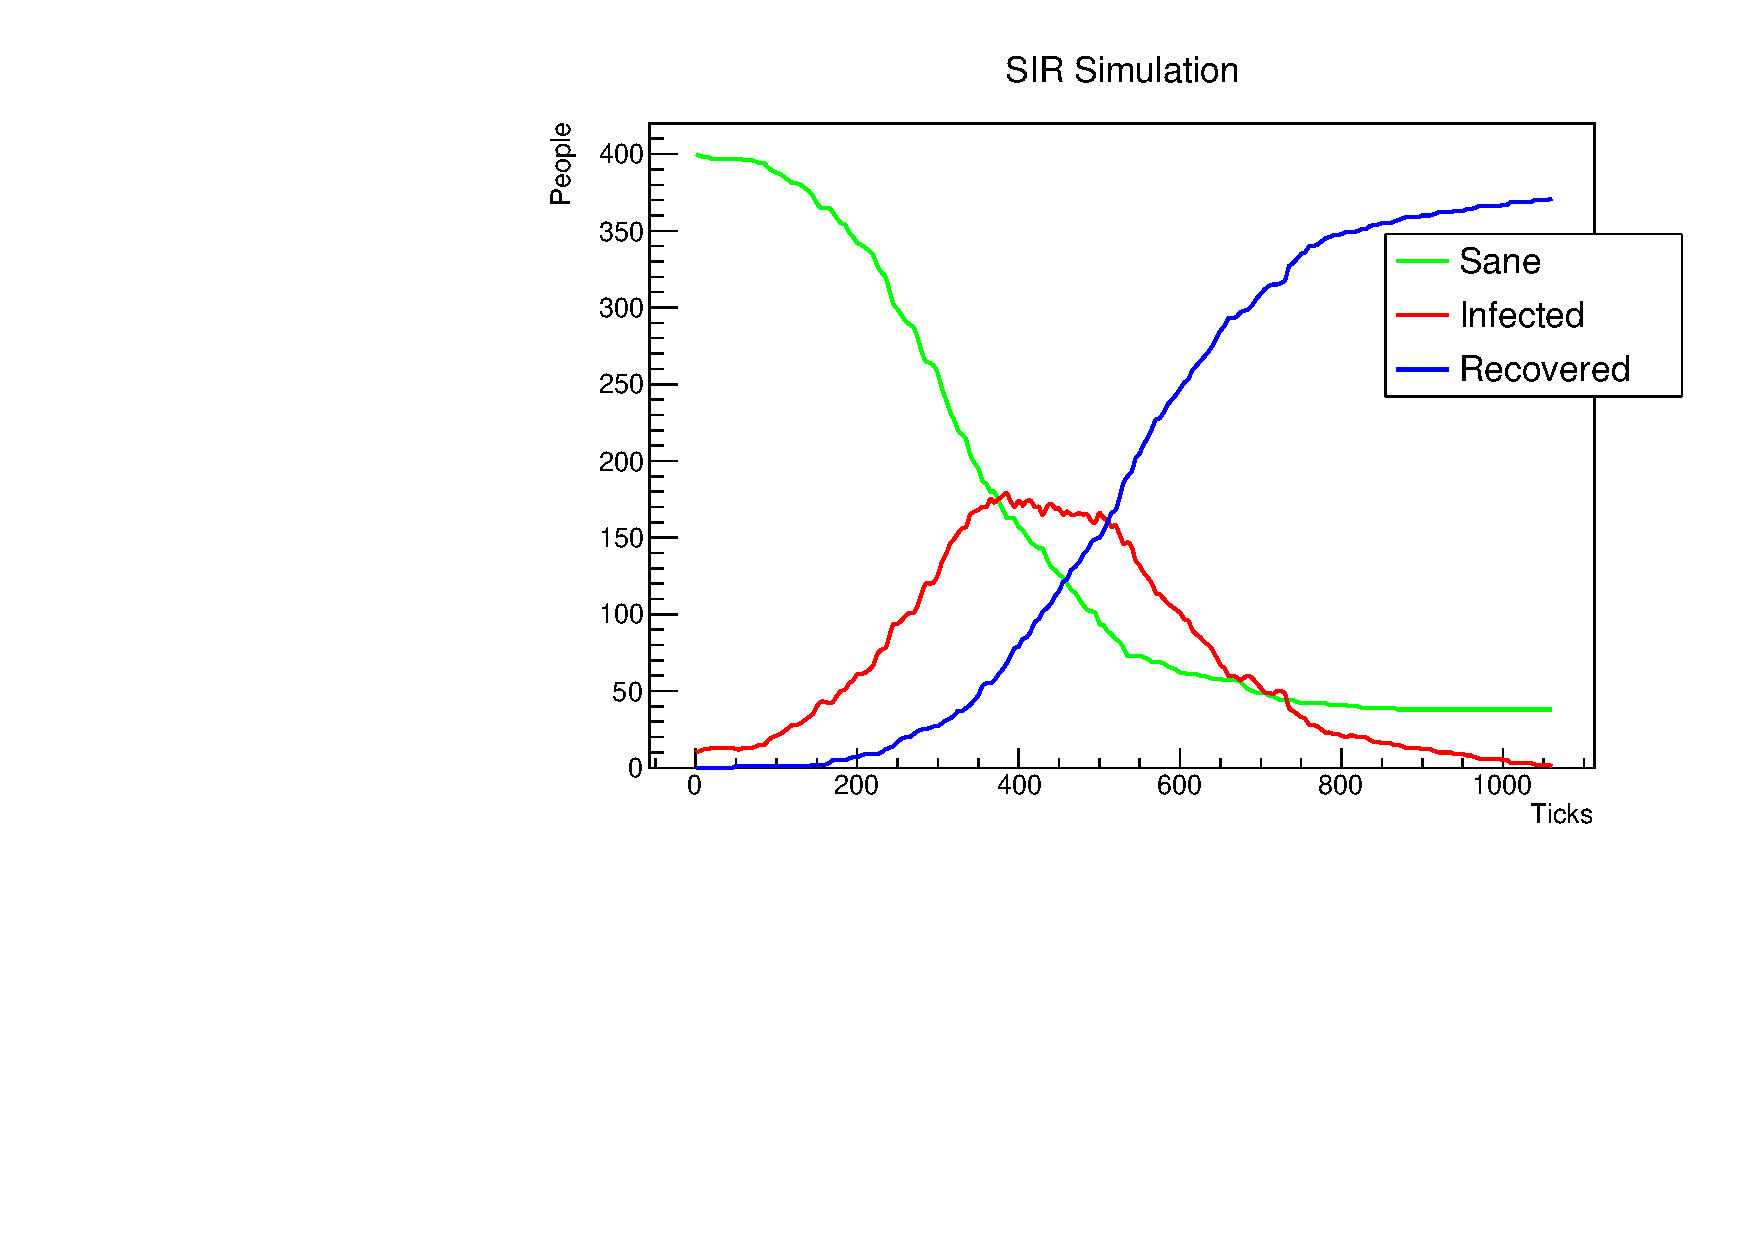
\includegraphics[width=0.5\textwidth]{images/simple_005.pdf}
    }
    \subfloat[][Probabilità: 0.08\label{fig:simple_008}]{
        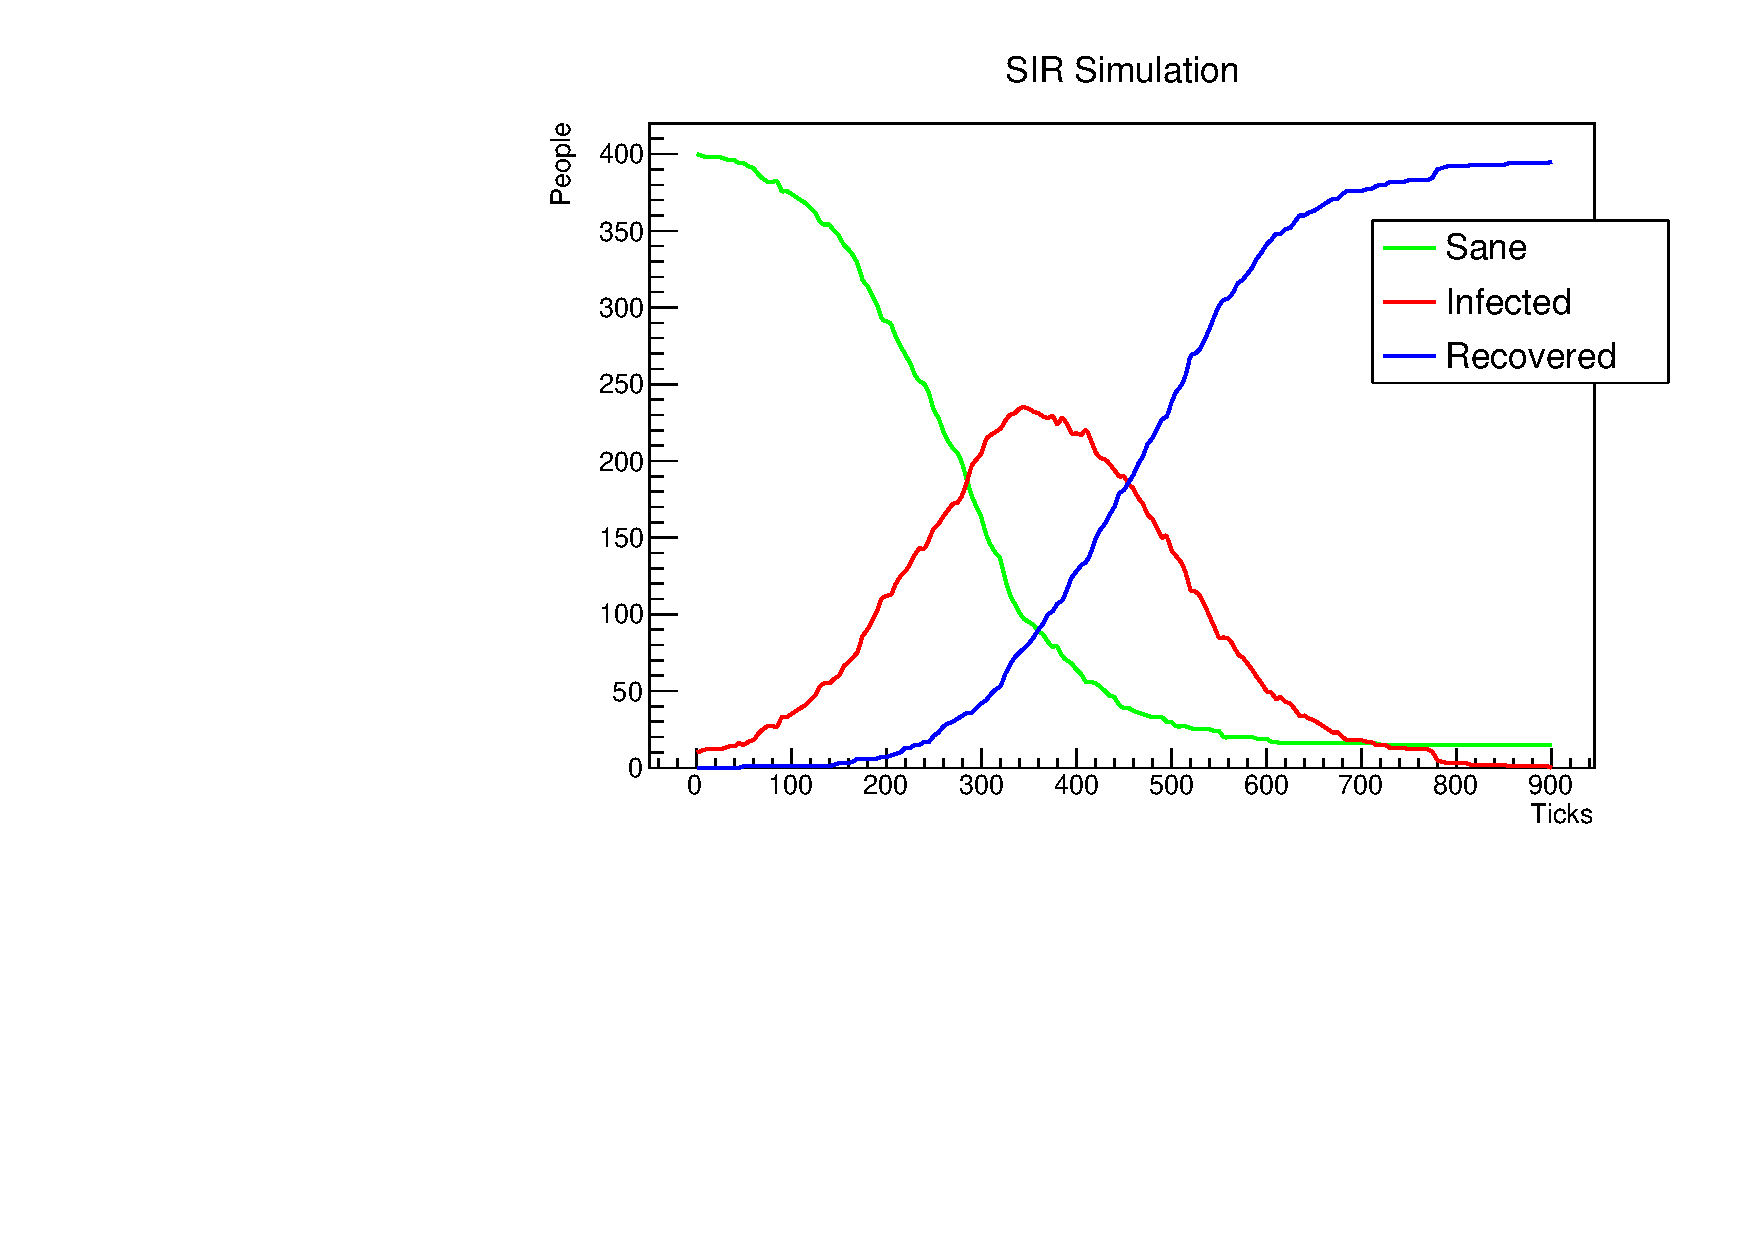
\includegraphics[width=0.5\textwidth]{images/simple_008.pdf}
    }
    \caption{Grafici di una simulazione con Simple Infection al variare della probabilità di infezione}
\end{figure*}

\begin{figure*}[p]
 \subfloat[][Size: 400\label{fig:simple_400}]{
        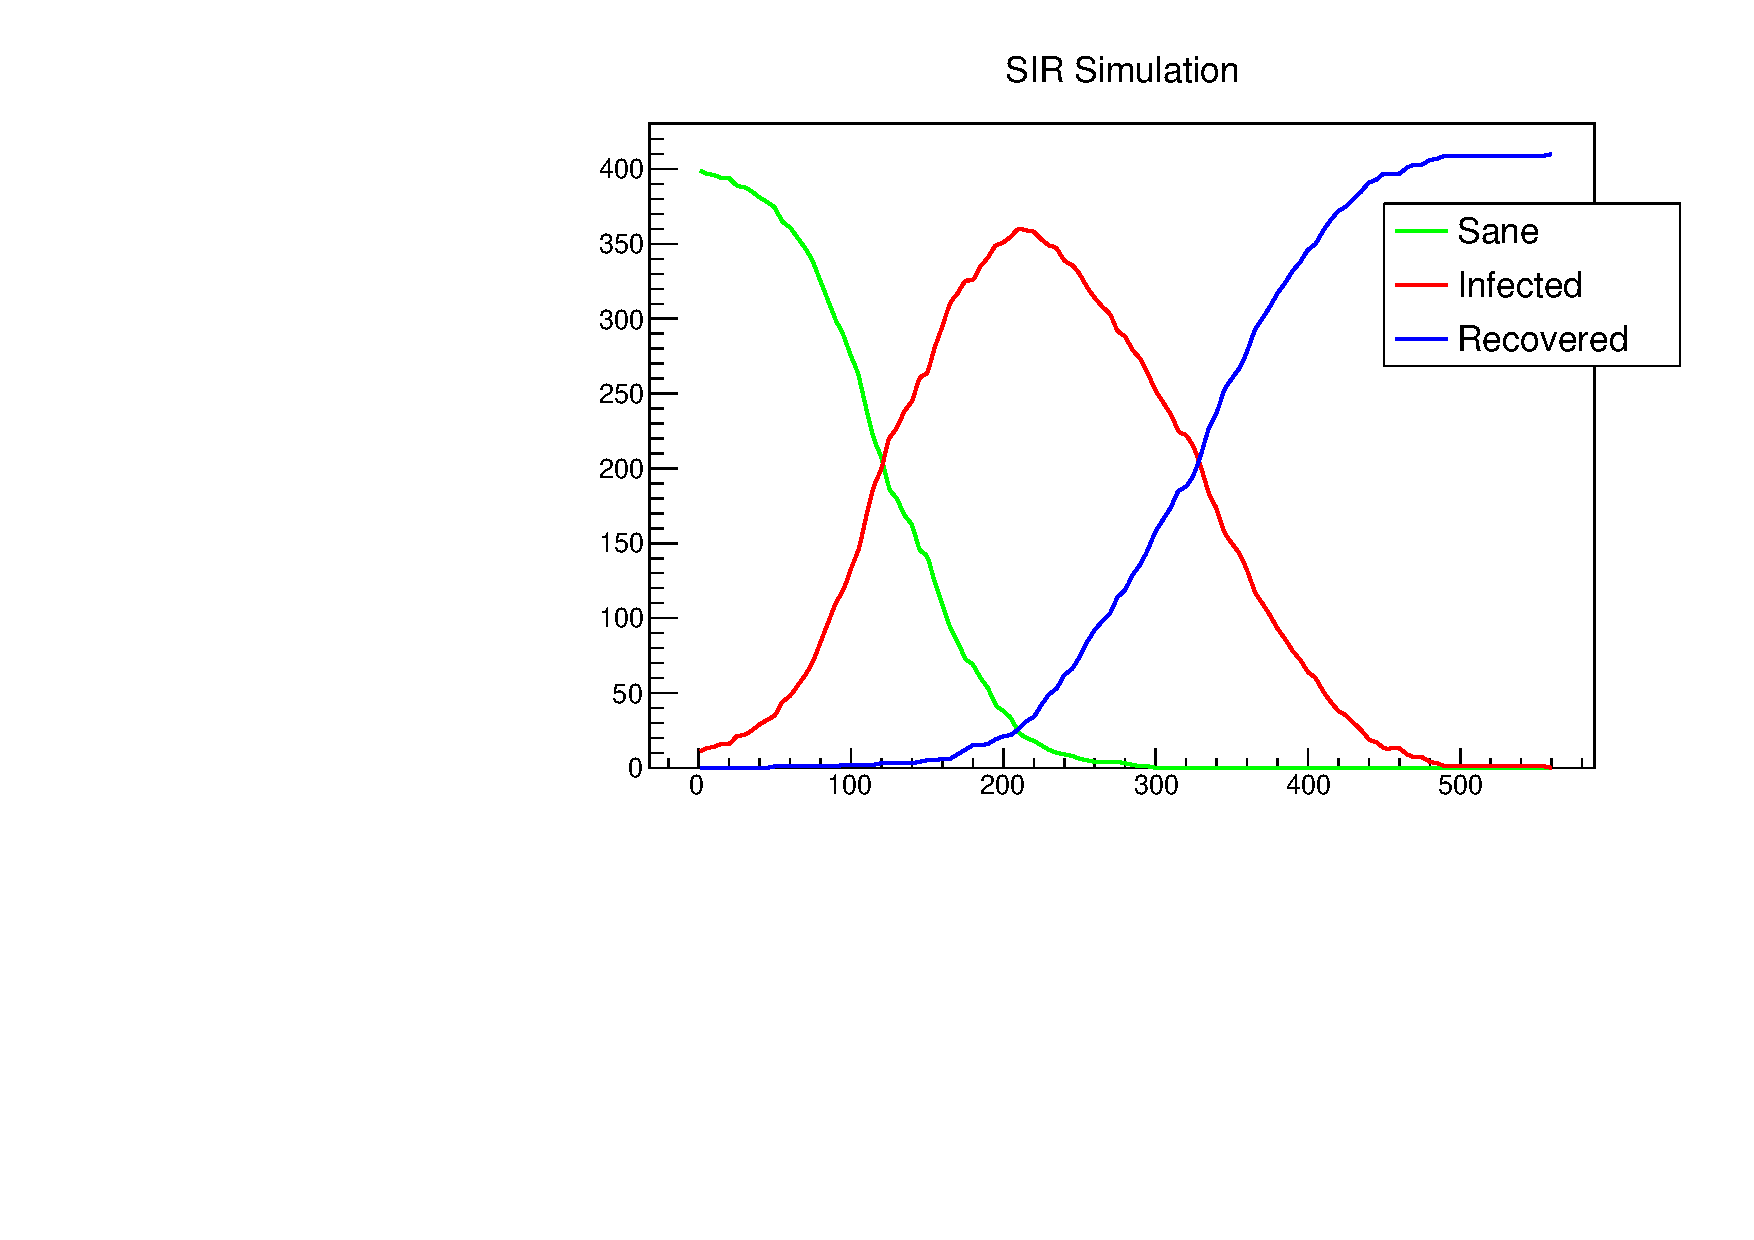
\includegraphics[width=0.5\textwidth]{images/simple_400.pdf}
    }
    \subfloat[][Size: 800\label{fig:simple_800}]{
        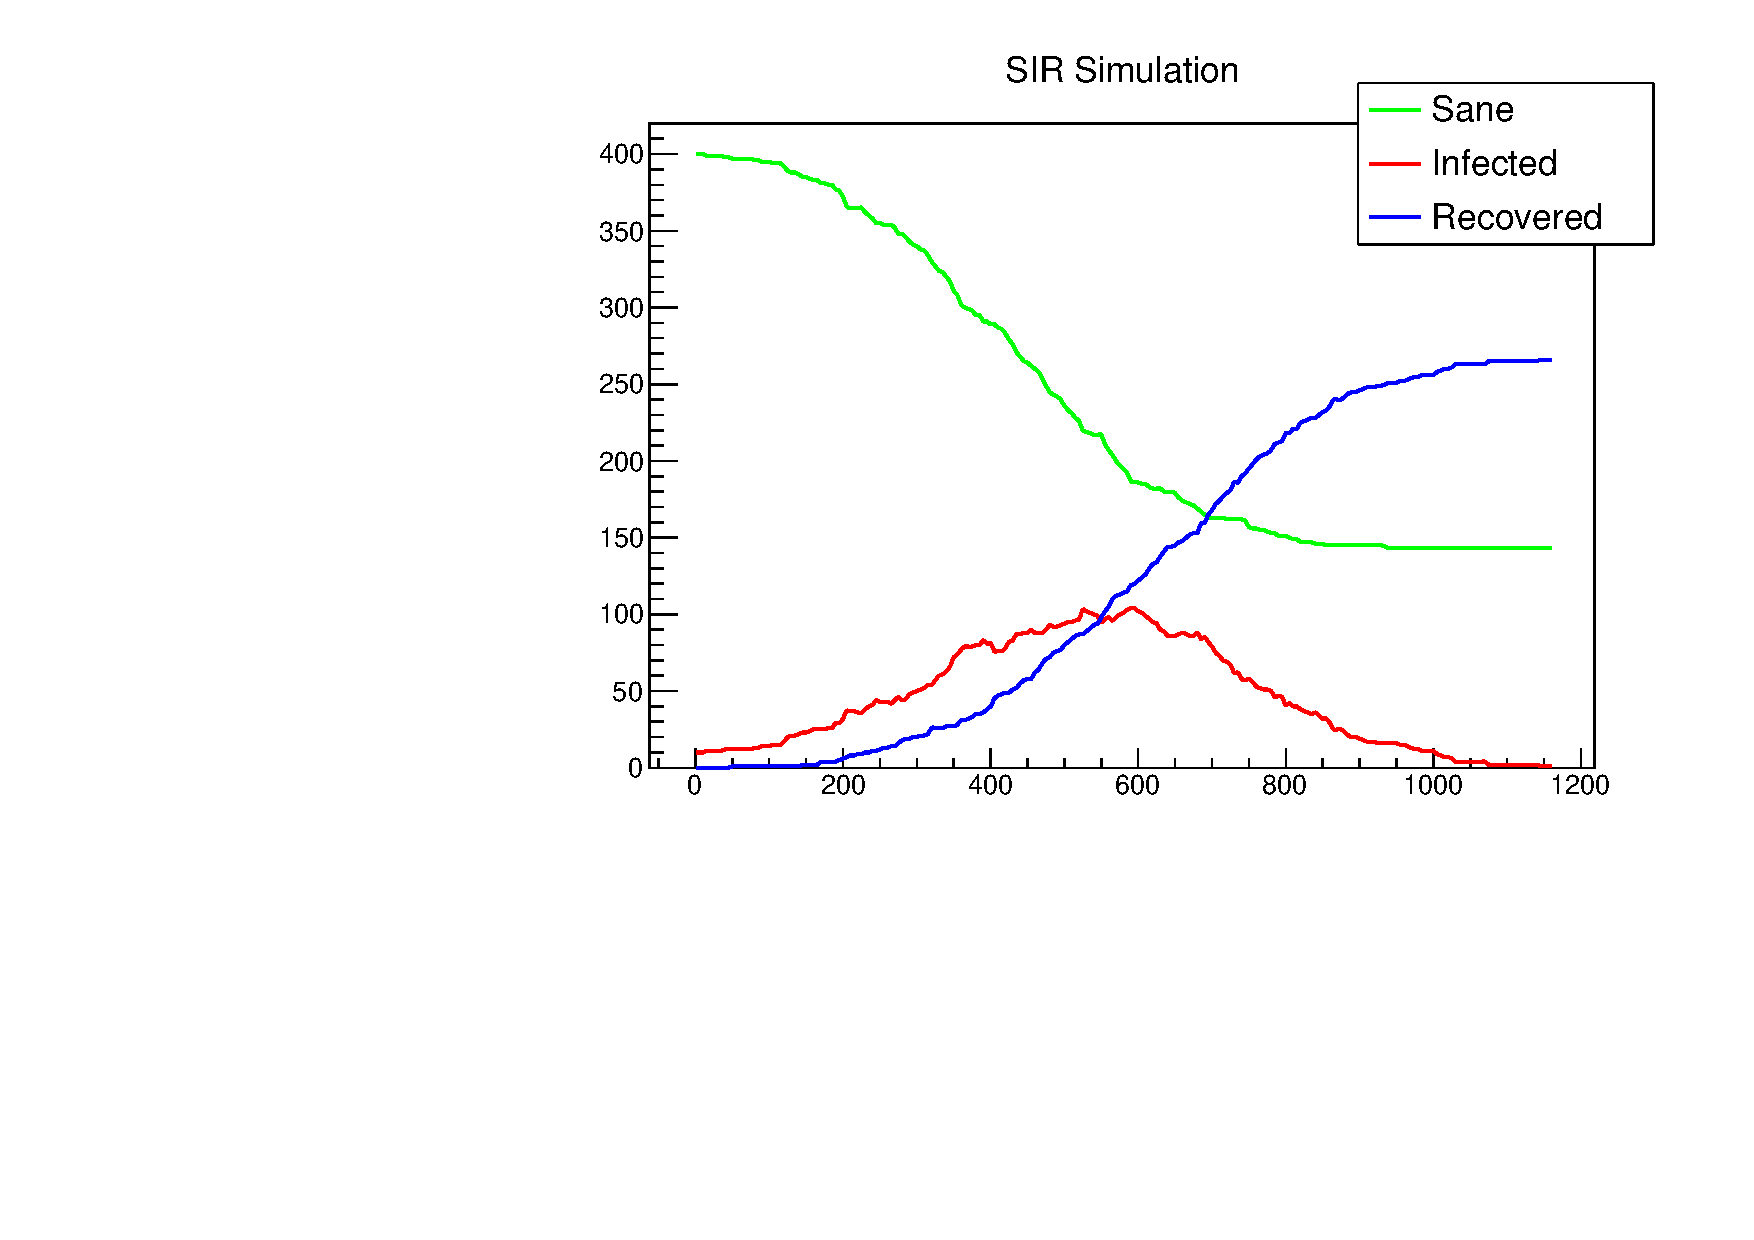
\includegraphics[width=0.5\textwidth]{images/simple_800.pdf}
    }
    \caption{Grafici di una simulazione con Simple Infection al variare della dimensione dell'ambiente}
\end{figure*}

\begin{figure*}[p]
    \centering
    \subfloat[][Senza quarantena\label{fig:incubation_005}]{
        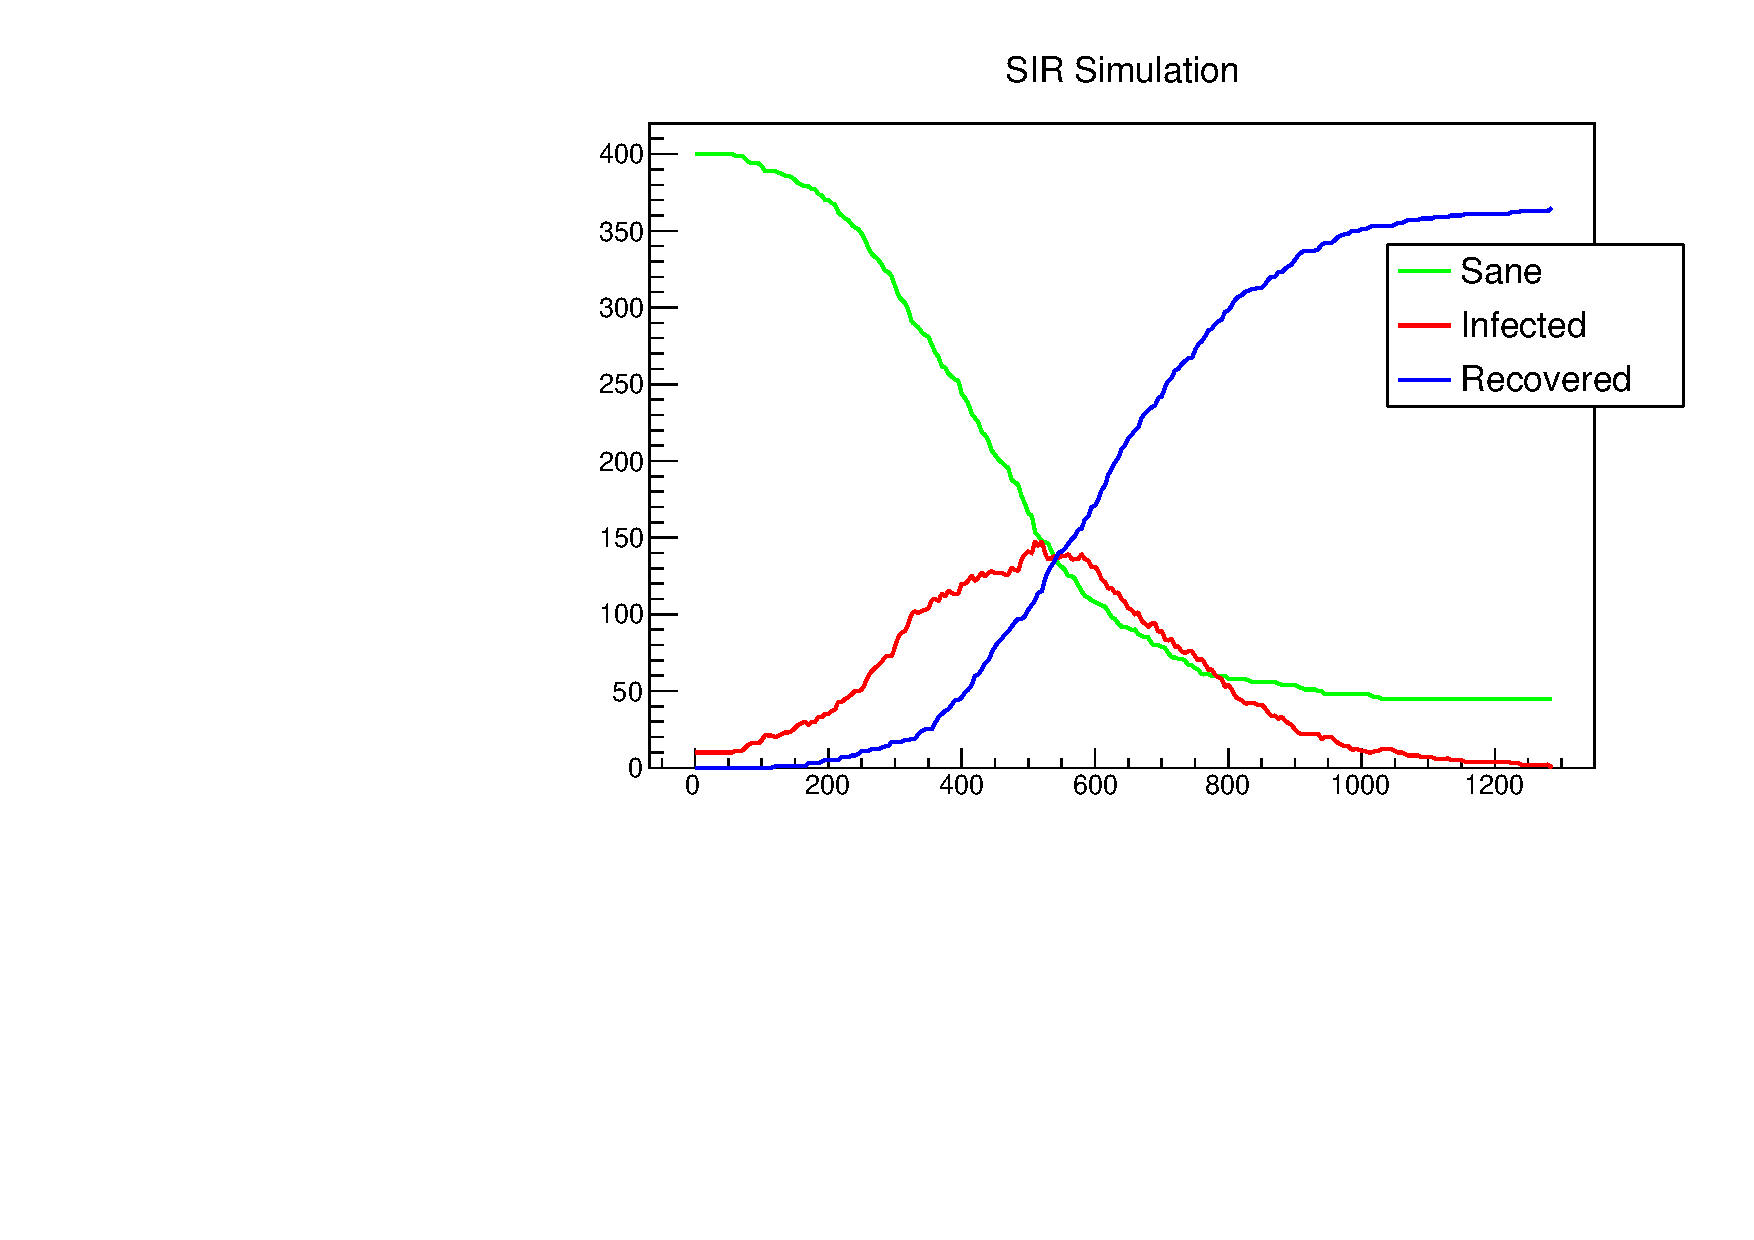
\includegraphics[width=0.5\textwidth]{images/incubation_005.pdf}
    }
    \subfloat[][Con quarantena\label{fig:quarantine}]{
        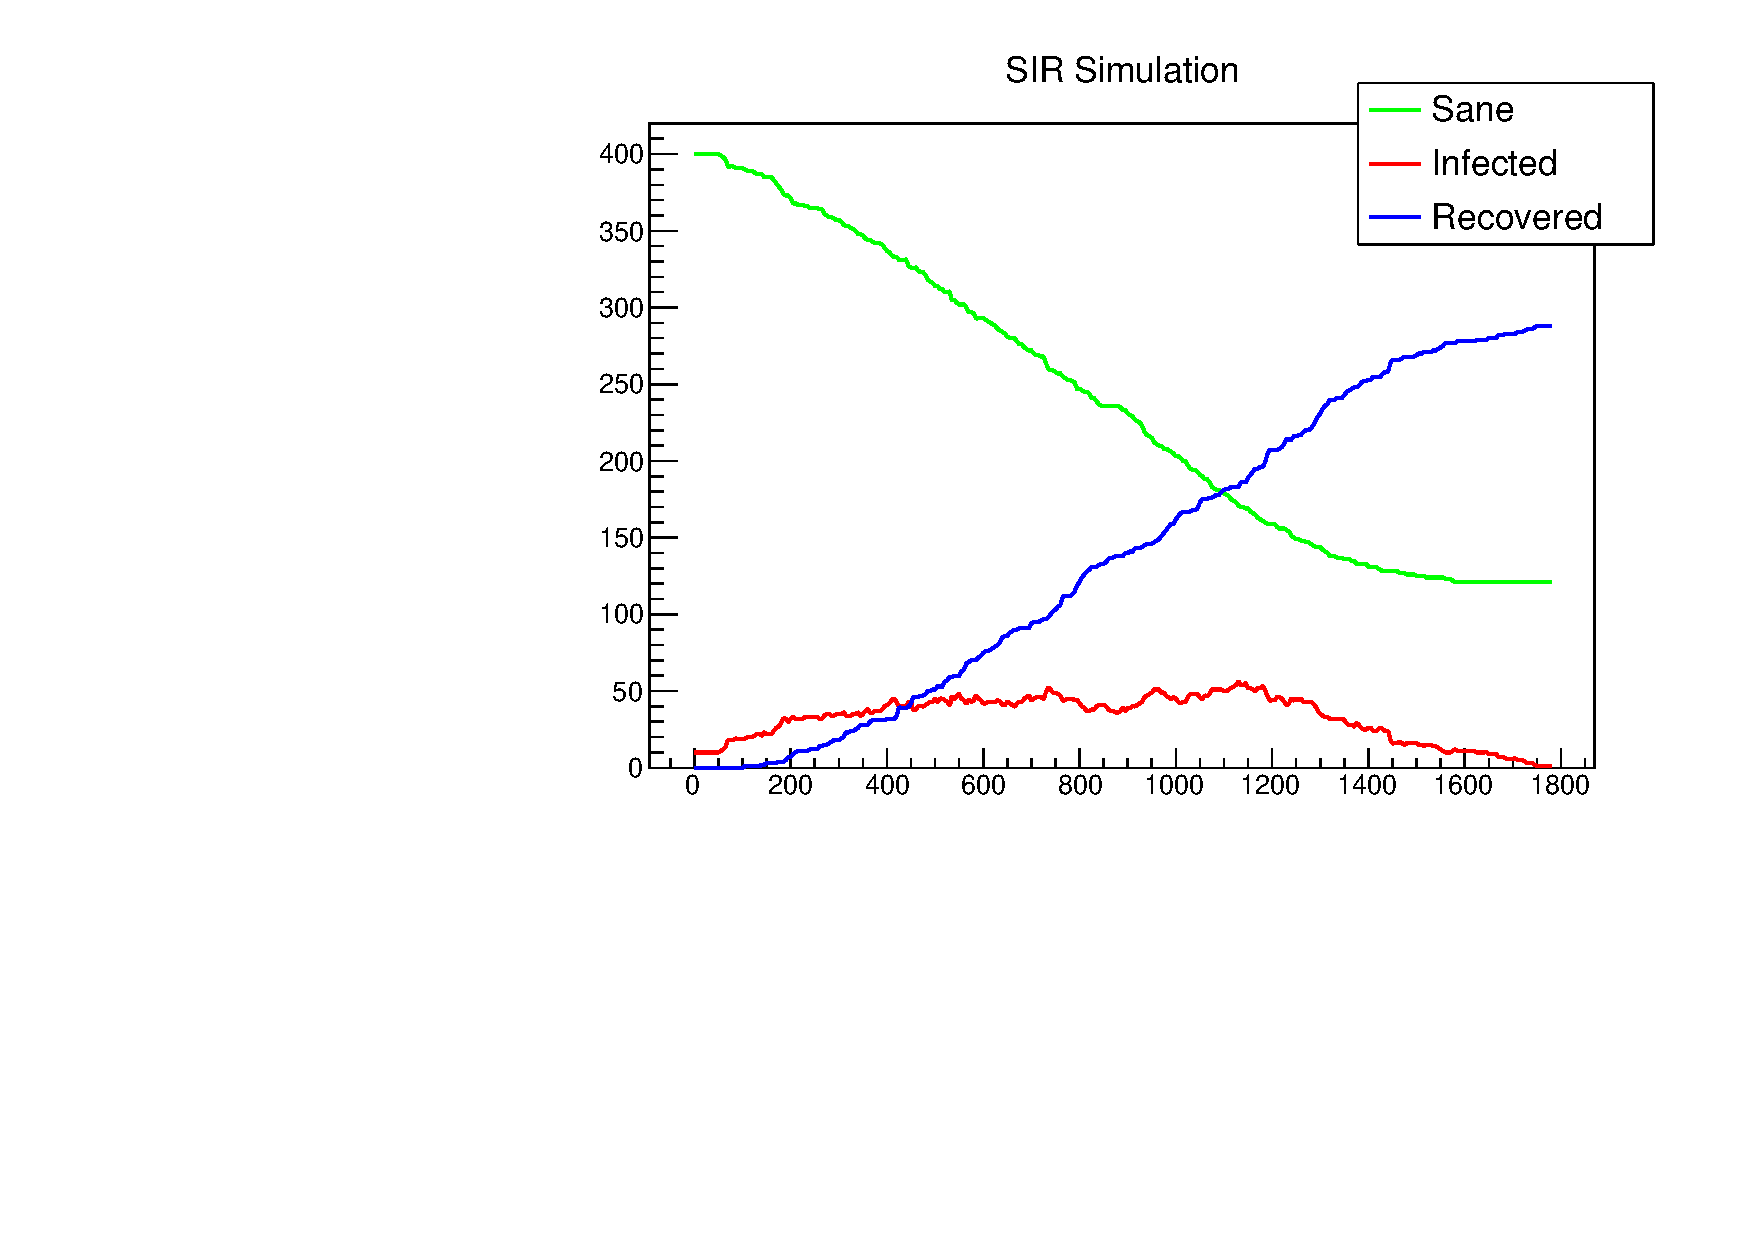
\includegraphics[width=0.5\textwidth]{images/quarantine.pdf}
    }
    \caption{Grafici di una simulazione con Incubation Infection con e senza la possibilità di essere costretti alla quarantena}
\end{figure*}

\section{Strategie di testing}

\end{document}